\chapter{Machine Learning Methods}\label{ch:3}
This chapter will treat the machine learning methods applied in this thesis. The subsection: \ref{Chapter:PUL} will discuss the Positive Unlabeled Learning (PUL) strategy for \textit{training} of our prediction model, in the following: \ref{Chapter:SVM} section, this thesis will point out the  idea of Support Vector Machines (SVM) including an introduction into the theoretical parts. The subjecting chapter: \ref{Chapter:OC-SVM} approach on One Class SVM, it will cover the concept and the gaps in respect to the ordinary SVM. At the end of this chapter, the subsection: \ref{Chapter:Ensemble} will introduce the concept of Ensambles in scope of machine learning especially to improve the classification accuracy.

The purpose of the following introduction is:
\begin{itemize}
    \item Understand the core concept of the particular algorithms.
    
    \item Get a brief understanding of the theoretical concepts driving the algorithms.
    
    \item Became familiar with the possible tuning options that the algorithms contain and be able to track the motivation of adjusting them.
\end{itemize}
One last note before starting: the theoretical concepts will be presented in an aggregated form. The goal is to provide only the information necessary to follow up in the further chapter. 

\section{Positive Unlabeled Learning}\label{Chapter:PUL}
Faced with the fact that the anomalous class examples are sparsely available but we still prefer to use supervision we have to label at least an subset of our underlying data. \textit{Positive Unlabeled Learning (PU Learning)} is an classification approach where the data is separated in two sets: \(P\) contained positive in our case examples that are labeled as non anomalous and \(U\) that can contain outliers as well as positive unlabeled data.

\section {Support Vector Machines (SVM)}\label{Chapter:SVM}

%http://stats.stackexchange.com/questions/63028/one-class-svm-vs-exemplar-svm
Support Vector Machines (SVM) \cite{Cortes;Vapnik:1995} is a state-of-the-art method with a solid background in statistical learning theory. It can be used for both classification and regression tasks. What distinguishes an SVM from other methods is a better ability to deal with high dimensional data and the guarantee of the globally optimal solution. The solution an SVM produces is sparse in many cases as only a fraction of training set instances is relevant for the task at hand. These instances, called support vectors, lie close to a hyperplane separating data into classes. Thus, an SVM tries to transform nonlinearly separable classes into linearly separable ones because the latter case is simpler to solve than the former. Without loss of generality and for the purpose of this thesis, only one or two classes are assumed to be present in the data.

Let us assume that we are given a data set as
\[  S = \{(x_1,y_2), (x_2,y_2), ...,(x_n,y_n) \} \; x_i \in \mathbf{R^d} \; y_i \in \{-1,1\}, \]
where \( x_i\) is the \( i-\)th input instance or data point and \( y_i\) is its class label. Thus, \(x_i\) is a \(d-\) dimensional column vector whereas \( y_i\) is a scalar.

A hyperplane that splits the data into two classes can be represented with the following equation:
\[\vec{w}^Tx + b = 0, \] 
where \(\vec{w}\) is a \textit{weight vector} determining the direction perpendicular to the hyperplane and \(b\) a \textit{bias} responsible for moving the hyperplane parallel to itself (see also~\label{fig:hyperplane1}.

\begin{figure}[h!]
    \centering % Picture from Oleg's book, do not forget the reffs!
    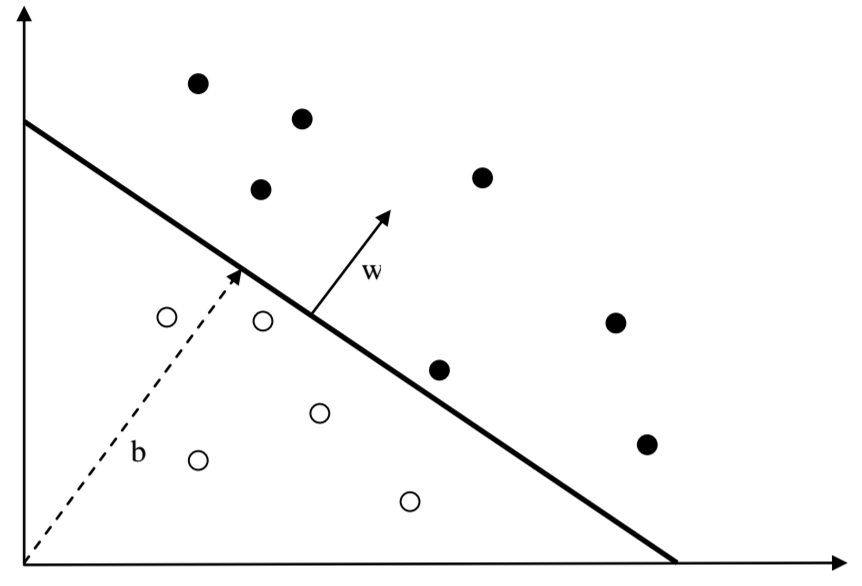
\includegraphics[scale=0.4]{Graphics/svm1.png}
    \caption{Hyperplane for separating 2-dimensional data.}
    \label{fig:hyperplane1}
\end{figure}

However, classes in the input space are often not linearly separable, which means that a linear classifier is not a good option in such a case. In the case of SVMs a solution is to project the original data into another, often a higher dimensional space \(x \mapsto \phi(x) \), where classes would more likely be linearly separable. Figure~\ref{fig:hyperplane2} shows an example of input space \(X\) where data cannot be separated by a linear function. However after applying the mapping function \(\phi\) to each data point in \(X\), the data become well separable in a \textit{feature space} \(F = \{ \phi(x)\; | \; x \in X\}\).
\begin{figure}[h!]
    \centering
    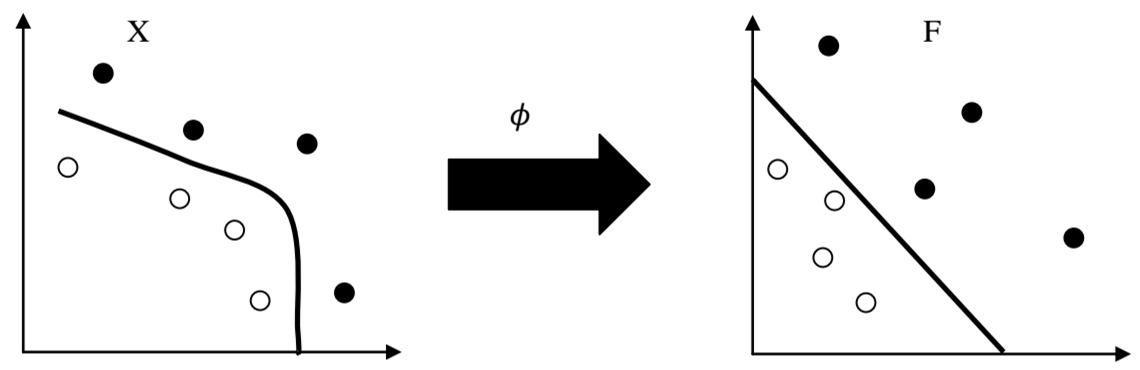
\includegraphics[scale=0.6]{Graphics/svp-separation.png}
    \caption{Mapping data into feature space.}
    \label{fig:hyperplane2}
\end{figure}

Thus, a straightforward solution seems to transforms data into a feature space where a linear classifier can be built. These two operations are combined with the help of a kernel function. The typical kernel functions are:
\begin{itemize}
            \item \(K(x,z) = x'z \)
            \item \(K(x,z) = (\tau + x'z)^b\)
            \item \(K(x,z) = exp(-\sigma||x-z||^2)\)
\end{itemize}

As one can see, the kernel representation eliminates the necessity to map each input individually: the inputs never appear isolated but in the form of inner products between pairs of inputs. Because of this, we don't need to know the underlying feature map! Also the dimensionality of the feature space does not affect the computation as the inner product is a number. As a result, the only information that is necessary is a \(n\times n\) kernel matrix.

Kernels provide one pillar of SVMs. The other is the optimization theory as the SVM solution is formulated as an optimization task, subject to certain constraints. The primal optimization problem where \( w \) and \( b \) are involved is difficult to solve due to inequality constraints. Instead the dual problem, based on  Lagrangian theory \footnote{Lagrangian theory is a basic mathematical tool for constrained optimization of differentiable functions, especially for nonlinear constrained optimization \cite{Li:2008}.} transforms the task into a quadratic programme where the function to be optimized is quadratic while the constraints are all equalities rather than inequalities. The solution of such a problem is known to be unique and global. It is also sparse by implying that only a small fraction of the original data matters for class separation, which results in a very efficient classifier.

Below both primal and dual optimization problems are given. The maximal (or hard) margin problem assumes two classes are only linearly separable in the feature space. To remedy its deficiency, the soft margin problem are then presented that works with nonlinearly separable classes.

The maximal margin:

Primal problem:

\[\textrm{minimize: } \vec{w} \vec{w},\] 
\[\textrm{subjects to: } y_i(\vec{w}\vec{x_i} + b) \geq +1, i = 1, ...,l \] 

Dual problem:
\[\textrm{\textit{maximize: } } W(a) =  \sum_{i=1}^{l} a_i \; - \frac{1}{2}\sum_{i,j = 1}^{l}a_i a_j y_i y_j \vec{x_i}^T \vec{x_j}, \] 

\[\textrm{subjects to: } \sum_{i=1}^{l}a_i y_i = 0, a_i \geq 0, i = 1,...,l.   \] 

The 2-norm soft margin:

Primal problem:

\[\textrm{minimize: } \vec{w} \vec{w} + C \sum_{i=1}^{l} \xi^2_i \textrm{over} \xi,\vec{w},b\] 
\[\textrm{subjects to: } y_i(\vec{w}\vec{x_i} + b) \geq 1 - \xi_i,, i = 1, ...,l \] 

Dual problem:
\[\textrm{maximize:} W(a) =  \sum_{i=1}^{l} a_i \; - \frac{1}{2}\sum_{i,j = 1}^{l}a_i a_j y_i y_j \Big( K\vec{x_i}^T \vec{x_j}) + \frac{1}{c}\delta_i_j \Big), \] 

\[\textrm{\textit{subjects to: }} \sum_{i=1}^{l}a_i y_i = 0, a_i \geq 0, i = 1,...,l.   \] 


The 1-norm soft margin:

Primal problem:
\[\textrm{minimize: } \vec{w} \vec{w} + C \sum_{i=1}^{l} \xi_i \textrm{over} \xi,\vec{w},b\] 
\[\textrm{subjects to: } y_i(\vec{w}\vec{x_i} + b) \geq 1 - \xi_i,\xi_i \geq 0, i = 1, ...,l. \] 

Dual problem:

\[\textrm{maximize: } W(a) =  \sum_{i=1}^{l} a_i \; - \frac{1}{2}\sum_{i,j = 1}^{l}a_i a_j y_i y_j (\vec{x_i}^T \vec{x_j}) , \]
\[\textrm{subjects to: } \sum_{i=1}^{l}a_i y_i = 0,C \geq a_i \geq 0, i = 1,...,l.   \] 

For the hard margin classifier SVM introduce additional classification hyperplanes:
\[H_1 : \vec{w}^Tx_i^- + b= -1\] 
\[H_2 : \vec{w}^Tx_i^+ + b= +1\] 
each of them cross at least the points of the particular classes which are the nearest points in respect to the separating hyperplane.
\begin{figure}[h]
    \centering
    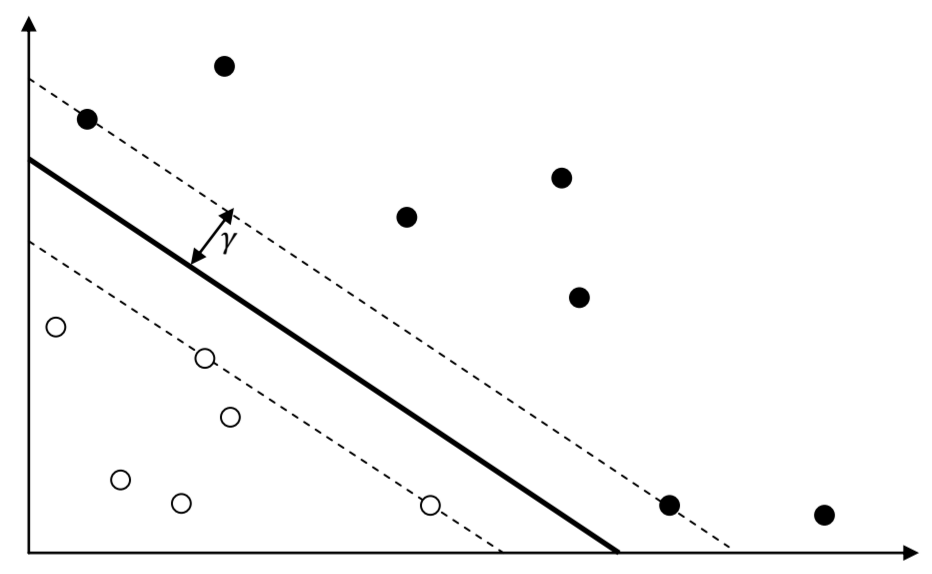
\includegraphics[scale=0.4]{Graphics/svm-margins.png}
    \caption{Separator hyperplane and two margin planes.}
    \label{fig:hyperplane3}
\end{figure}
The goal is to find the widest possible margin between the separator hyperplane \(H_0 \longleftrightarrow H_i\) and the classification hyperplanes. The margin is defined as an optimization problem:
\[ \textrm{\textit{maximize} } \frac{2}{||\vec{w}||} \mapsto \textrm{\textit{minimize} } \frac{||\vec{w}||}{2} \mapsto \textrm{\textit{minimize} } \frac{1}{2}||\vec{w}||^2\]
\[\textrm{With constraints:} \]
\[  y_1 = +1, \; \vec{w}^Tx_1 + b = \; \geq +1\]
\[  y_2 = -1, \; \vec{w}^Tx_2 + b = \; \leq -1\]
\[\textrm{Multiplying the constraints with each labels so both     constraints can be substituted to a single one:}\]
\[ y_i(\vec{w}^Tx_i + b) \geq +1\]
Solving constrained problems by using Lagrangian multipliers. The \textit{primal} optimization problem is defined as: 
\[\textrm{\textit{minimize} } L_p(\vec{w},a_i,b) = \; \frac{1}{2}||\vec{w}||^2 - \; \sum_{i=1}^{n} a_i(y_i(\vec{w}^T x_i +b) - 1) \]
\[\textrm{such that } a \geq 0 \]
Subjecting the primal representation to the so called \textit{dual} representation which often turns to be easier to solve than the primal problem since handling inequality constraints directly is difficult.
%here link to Oleg's book.
\[\textrm{\textit{maximize} }  \sum_{i=1}^{n} a_i \; - \frac{1}{2}\sum_{i=1}^{n}\sum_{j=1}^{n}a_i a_j y_i y_j \vec{x_i}^T \vec{x_j} \]
\[\textrm{such that } a \geq 0, \textrm{ and } \sum_{i=1}^{n}a_i y_i = 0  \]
To solve the optimization problem we need to compute the dot product between all pairs of \(\vec{x_i}^T \vec{x_j}\). After solving the optimization problem we are able to define the decision rule to classify new data:
\[  f(x) = \vec{w}^T x + b = \sum_{i=1}^{n}a_i y_i x_i^T x + b \; \geq 0  \]
Where \(x_i\) are the support vectors and \(x\) is the test point. \newline

A quick summary of things we already discussed:
\begin{itemize}
    \item SVM classify the data by finding a optimal linear hyperplane which split the data in two or more classes.
    
    \item The algorithm of SVM can linear separate non linear data by casting it into a higher space with the kernel method.
    
    \item The core idea of SVM is to find a widest possible margin between separator hyperplane and the support hyperplanes. Bigger the margin better classification.
    
    \item Computing the biggest margin subjects to an optimization task in quadratic programming. The computation process can also be called \textit{training} in machine learning context.
\end{itemize}

As last but not least this chapter will introduce an important concept to optimize the results produces by SVM, called \textit{soft margin optimization}.

Most real world data consist \textit{noise} caused by overfitting (high complexity of input data), this can result in poor generalisation and negative affect the performance of SVM. The concept of soft margin optimization can be viewed as the relaxation of the hard margin constraint discussed above. First of all we introduce two \textit{slack} variables: \(\xi \) which allow some data to overlap the separation boundary see figure: \ref{fig:slackvariable} and \(C > 0\)  a positive scalar as the regularization parameter to control possible overfitting.
\begin{figure}[h!]
    \centering
    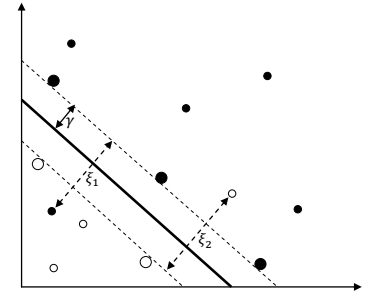
\includegraphics[scale=0.4]{Graphics/svm-slack-variable.png}
    \caption{Slack variable example.}
    \label{fig:slackvariable}
\end{figure}
Adding the slack variables to our optimization problem we get:

\[ min_{w,b,\xi} \;\; \frac{1}{2}w^Tw+C \sum_{i=1}^{l} \xi_i\]
\[ \textrm{such that } y_i(w^T\phi(x_i) + b) \geq 1 - \xi_i, \]
\[\xi_i \geq 0, i = 1,...,l \]

A final summary of this chapter:

\begin{itemize}
    \item SVM introduce a concept by dealing with noise called soft margin optimization.
    
    \item Soft margin optimization use slack variable \(\xi \) to allow data points overlap the separation boundary and \(C\) as upper bound to prevent overfitting. Both variables are the typical \textit{tuning parameter} in the common usage of SVM.
\end{itemize}


\subsection{One Class SVM}\label{Chapter:OC-SVM}
\textit{One Class SVM} is an SVM based classifier method. In contrast to the conventional SVM it has knowledge about only one class inside the data sample. 

\section{Ensemble SVM}\label{Chapter:Ensemble}
\textit{Ensamble SVM} is an approach to combine multiple SVM Algorithms. The general idea of sequential ensembles is to provide a better understanding of the data, so as to enable a more refined execution with either a modified algorithm or data set \cite{Aggarwal:2013} by applying the same or several classification algorithms on the same data and evaluating the results. Alternatively independent ensambles use different initialisations of same algorithm or different sub sets of underlying data. The results can be combined to obtain an more robust outlier score \cite{Aggarwal:2013}.

%http://www.outlier-analytics.org/odd13kdd/papers/slides_charu_aggarwal.p



% FAZIIIIIIT!!!!!


